\documentclass[10pt]{article}
\usepackage[margin=0.7in,top=0.55in,bottom=0.55in]{geometry}
\usepackage{graphicx}
\usepackage{xcolor}
\usepackage{booktabs}
\usepackage{enumitem}
\usepackage{titlesec}
\usepackage[hidelinks]{hyperref}
\usepackage{array}
\usepackage{parskip}

\definecolor{accent}{HTML}{2A78D6}
\definecolor{warncol}{HTML}{EB6834}
\definecolor{inksoft}{HTML}{52514E}
\definecolor{muted}{HTML}{898781}
\definecolor{rule}{HTML}{E1E0D9}

\titleformat{\section}{\large\bfseries}{}{0pt}{}
\titlespacing*{\section}{0pt}{8pt}{3pt}
\titleformat{\subsection}{\normalsize\bfseries\color{inksoft}}{}{0pt}{}
\titlespacing*{\subsection}{0pt}{6pt}{2pt}

\setlength{\parindent}{0pt}
\setlength{\parskip}{3pt}
\pagestyle{empty}

\begin{document}

{\LARGE \bfseries AR1 Simulation Comparison --- Free-Intercept LDSC, Reference-Panel Scenarios}

\vspace{2pt}
{\color{inksoft} {\small\ttfamily n=500, m=1000, AR1 $\rho$=0.3, $\sigma_s$=0.3, 100 reps per F$_{ST}$}}

\vspace{3pt}
\noindent\rule{\linewidth}{0.4pt}

\section*{Scope of this report}
\begin{itemize}[leftmargin=14pt, itemsep=1.5pt, topsep=1pt]
  \item This is a companion to the main R-vs-Python comparison report, restricted to the \textbf{reference-panel scenarios} (Sections 2--3 of the original report) and to the \textbf{free-intercept estimators only}.
  \item R has a single free-intercept estimator, \texttt{res\_reg\_free\_ref}. Python has \textbf{two} free-intercept LDSC variants: \texttt{h2\_ldsc\_nw} (no regression weights) and \texttt{h2\_ldsc\_reg} --- labeled here \texttt{h2\_ldsc\_free} --- (the standard LDSC weighted regression). Both are plotted against R's single free-intercept result.
  \item Fixed-intercept estimators are intentionally omitted from this report; see the main report for that comparison.
\end{itemize}

\section*{Section 2: Reference-panel LD scores, R's original (uncorrected) implementation}
Both sides use a separately-simulated reference panel (same generative process, independent individuals) for the LD score, reused across all 100 replicates. This is R's \emph{original} implementation, before bias correction was added to the R code --- R's reference-panel LD score has no correction term here, while Python's still applies its default bias correction. The only thing that changes between the two figures below is whether the reference panel's stratification draw $f$ is the \emph{same} one used to generate the 100 main replicates, or an independent one.

\begin{minipage}[t]{0.49\linewidth}
  \centering
  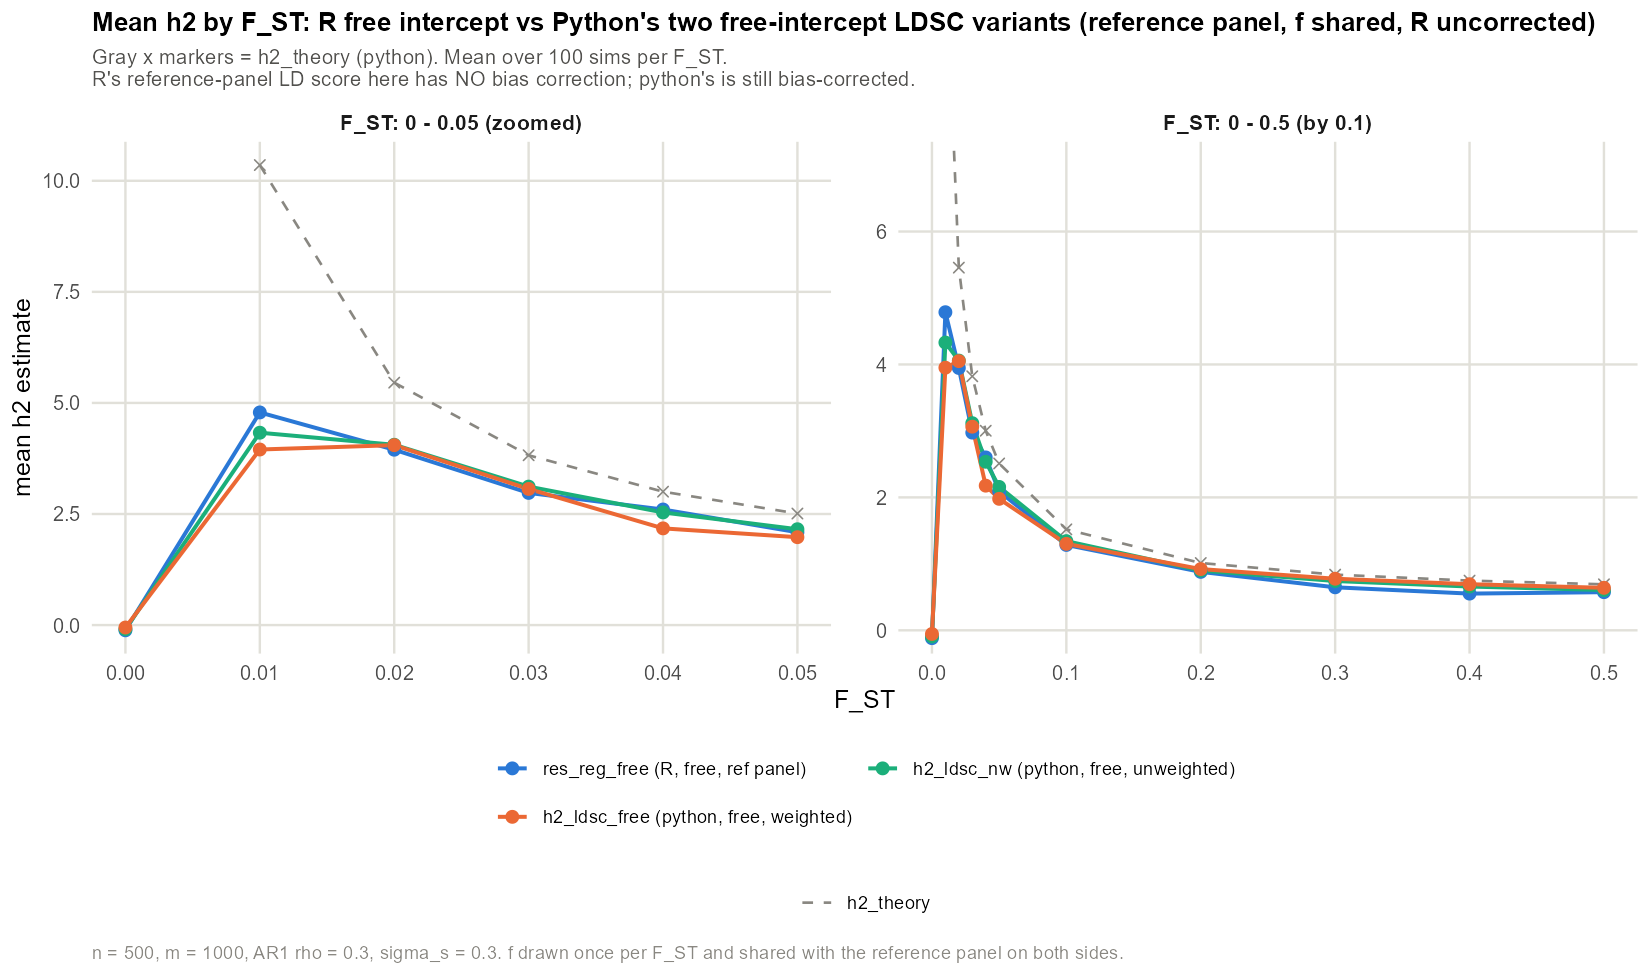
\includegraphics[width=\linewidth]{../figures/h2_by_fst_refpanel_fixedf_nobc_ldscfree.png}\\[2pt]
  {\footnotesize\color{inksoft}\textbf{Figure 1.} $f$ shared, R's reference LD score uncorrected.}
\end{minipage}
\hfill
\begin{minipage}[t]{0.49\linewidth}
  \centering
  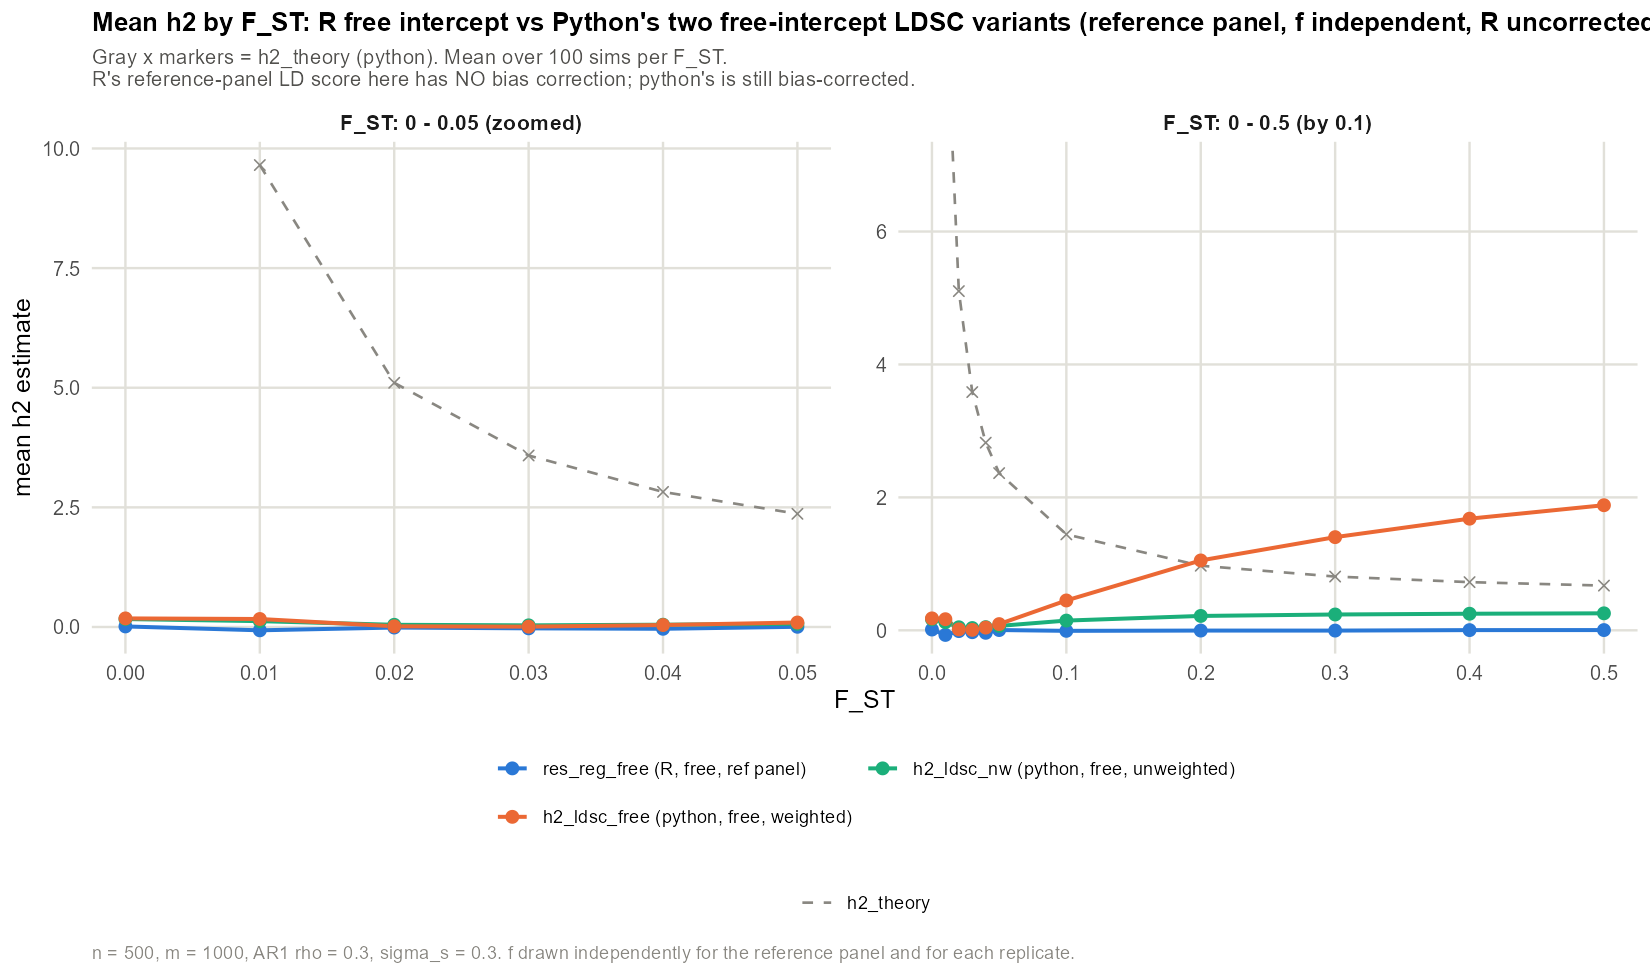
\includegraphics[width=\linewidth]{../figures/h2_by_fst_refpanel_indepf_nobc_ldscfree.png}\\[2pt]
  {\footnotesize\color{inksoft}\textbf{Figure 2.} $f$ independent, R's reference LD score uncorrected.}
\end{minipage}

\section*{Section 3: Adding bias correction to R's reference-panel LD score}
Same two configurations as Section 2 (f shared / f independent), but now R's reference-panel LD score gets the same bias-correction term Python already applies.

\begin{minipage}[t]{0.49\linewidth}
  \centering
  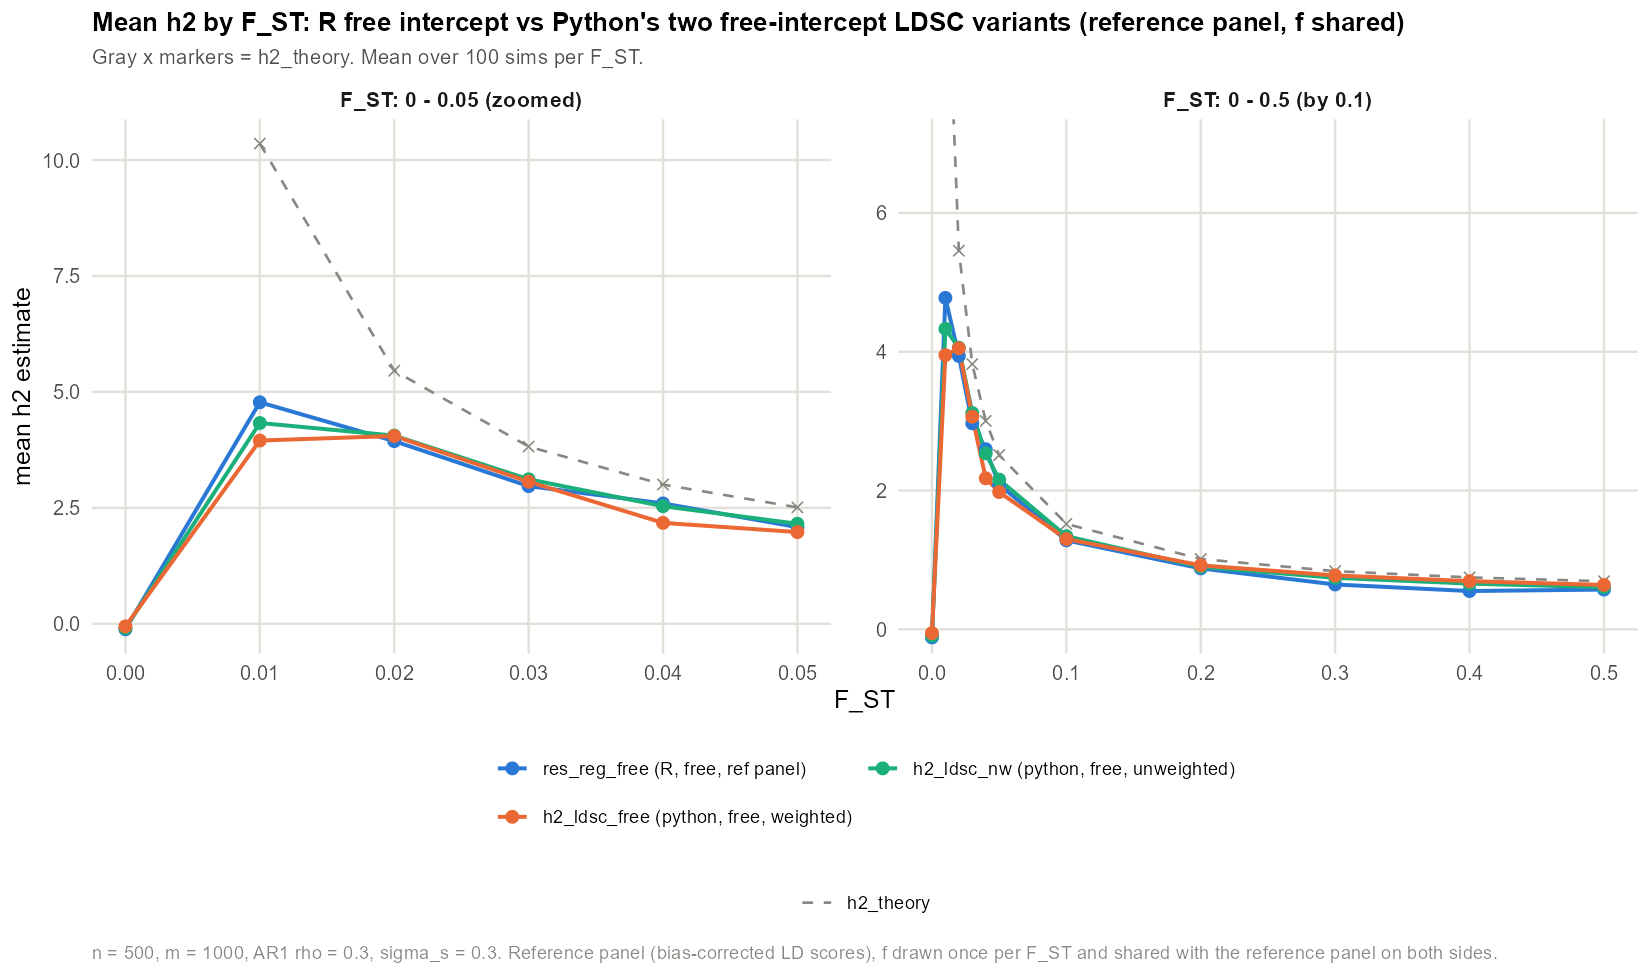
\includegraphics[width=\linewidth]{../figures/h2_by_fst_refpanel_fixedf_ldscfree.png}\\[2pt]
  {\footnotesize\color{inksoft}\textbf{Figure 3.} $f$ shared, R's reference LD score bias-corrected (matches Python's correction).}
\end{minipage}
\hfill
\begin{minipage}[t]{0.49\linewidth}
  \centering
  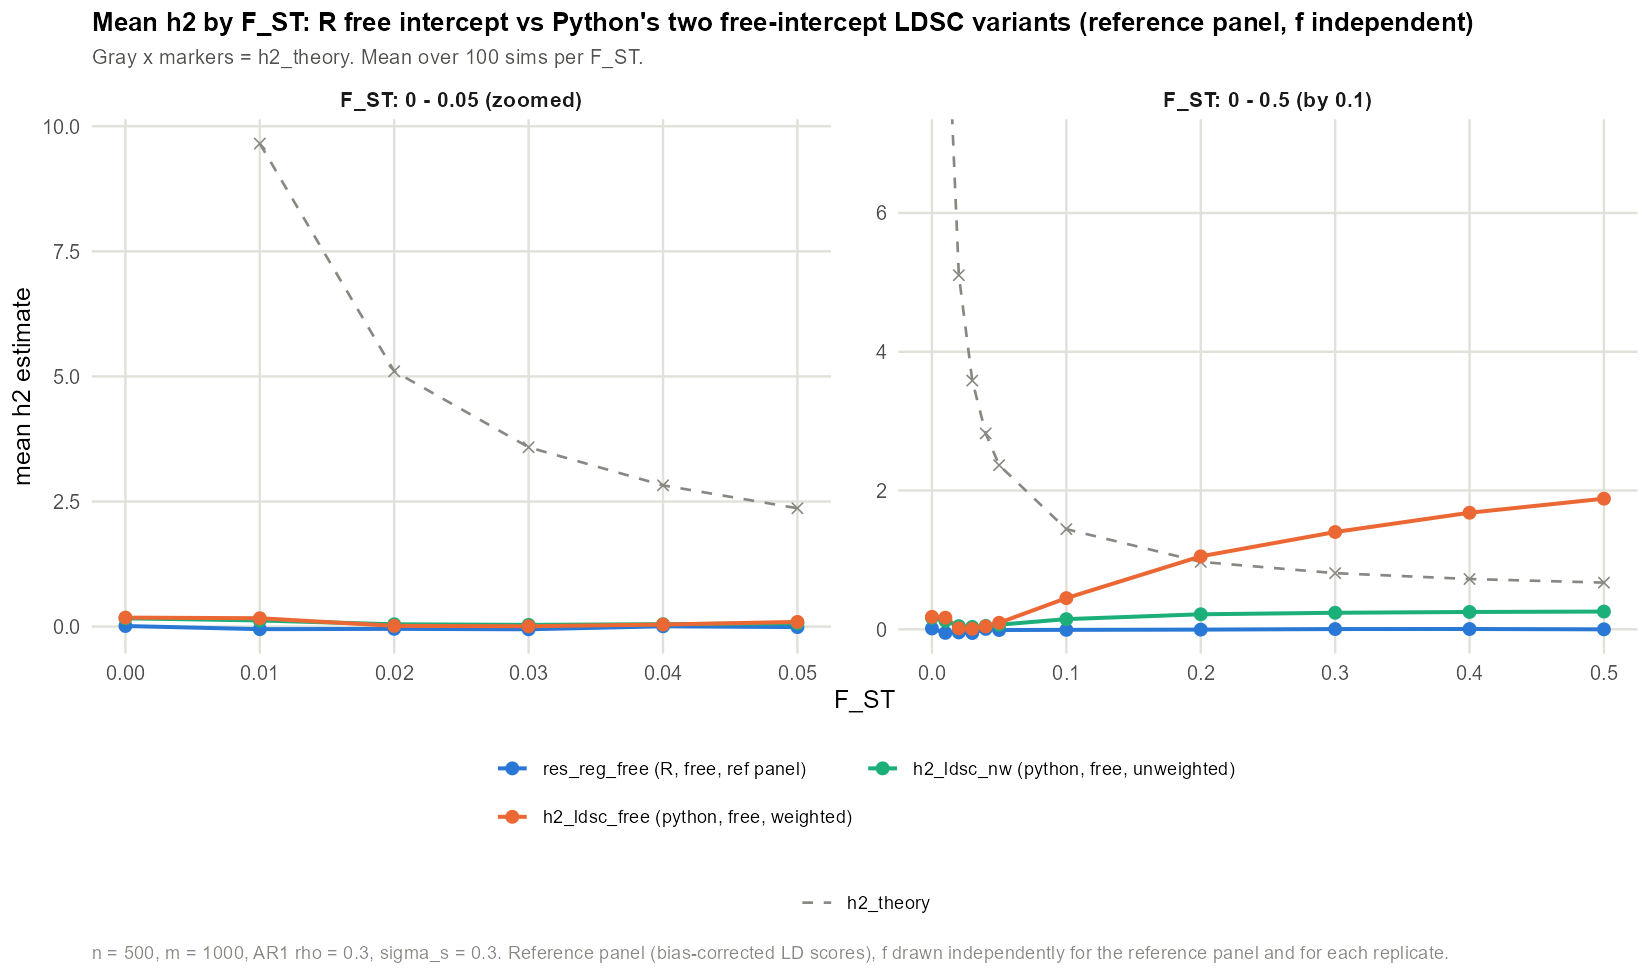
\includegraphics[width=\linewidth]{../figures/h2_by_fst_refpanel_indepf_ldscfree.png}\\[2pt]
  {\footnotesize\color{inksoft}\textbf{Figure 4.} $f$ independent, R's reference LD score bias-corrected.}
\end{minipage}

\vspace{4pt}
{\footnotesize\color{muted} See \texttt{report/report.tex} for the full comparison, including in-sample LD scores, fixed-intercept estimators, and the diagnosis of what drove each gap.}

\end{document}
